We applied the \textit{Cognitive Task Analysis} (CTA) methodology to explore individuals' knowledge and thought processes. Among the various CTA methodologies available, we selected the \textit{Goal-Directed Task Analysis} (GDTA), specifically focusing on Situation Awareness (SA) and the goals inherent in SA processes. 

\section{Initial GDTA Goal Tree}
The initial GDTA Goal Tree, shown in Figure 4.1, identified three Major-Goals. However, after an in-depth review and analysis, we concluded that the Major-Goal 1 \textbf{"Identify prior knowledge in the field of Cybersecurity"} can be integrated into the Major-Goal 2 \textbf{"Define and evaluate the knowledge required for Offensive Cybersecurity by monitoring students' progress"}. This conclusion was drawn from a comprehensive analysis of the sub-goals associated with Major-Goal 1.

Furthermore, the sub-goals of Major-Goal 1 have been reclassified as Level 2 elements, signifying their importance in the comprehension phase of the learning process. 

\begin{figure}[H]
    \centering
    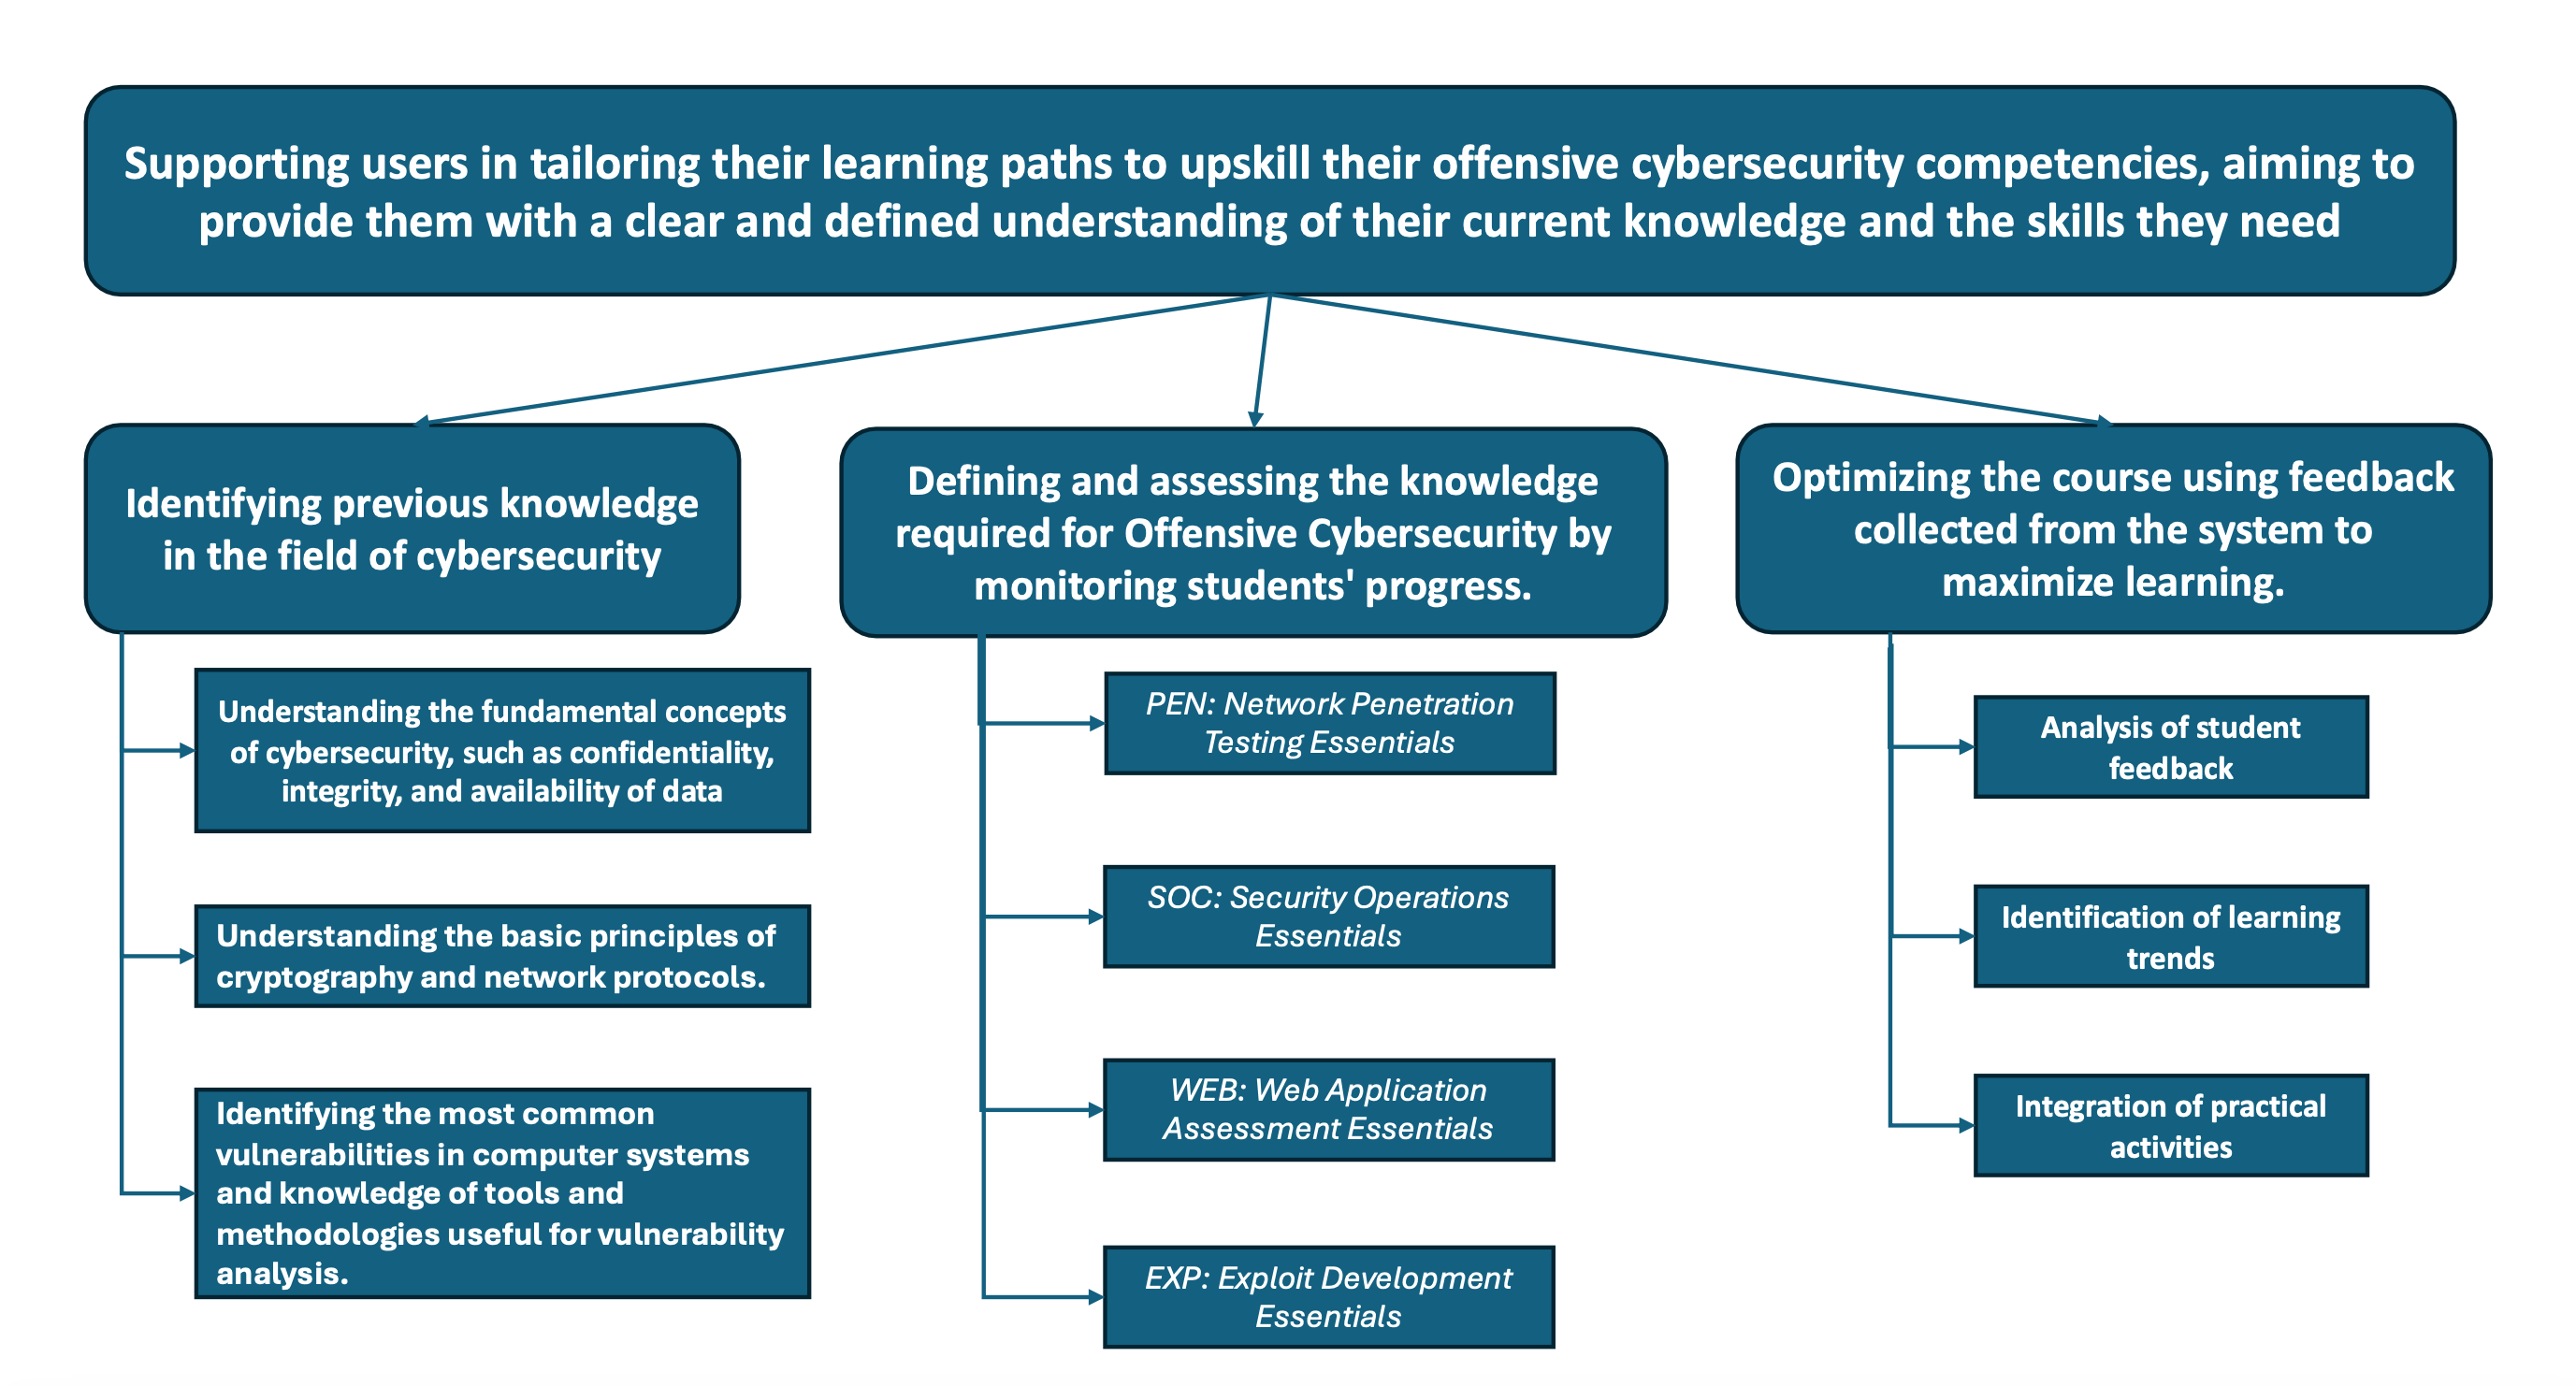
\includegraphics[width=\textwidth]{./assets/initialgdta.png}
    \caption{Initial GDTA Goal Tree}
    \label{fig:Initial GDTA}
\end{figure}

\newpage
\section{Final GDTA Goal Tree}
In Figure 4.2, we present our Final GDTA Goal Tree, which outlines the primary goals of the system and the sub-goals that contribute to their achievement. In particular, our GDTA Goal Tree supports users in adapting their learning paths to enhance their expertise in Offensive Cybersecurity.
The \textit{Overall Operator Goal} is broken down into two primary \textit{Major Goals} as shown in the picture below. Each Major Goal is further divided into \textit{SubGoals} that are essential for achieving the Major Goals. 

\begin{figure}[H]
    \centering
    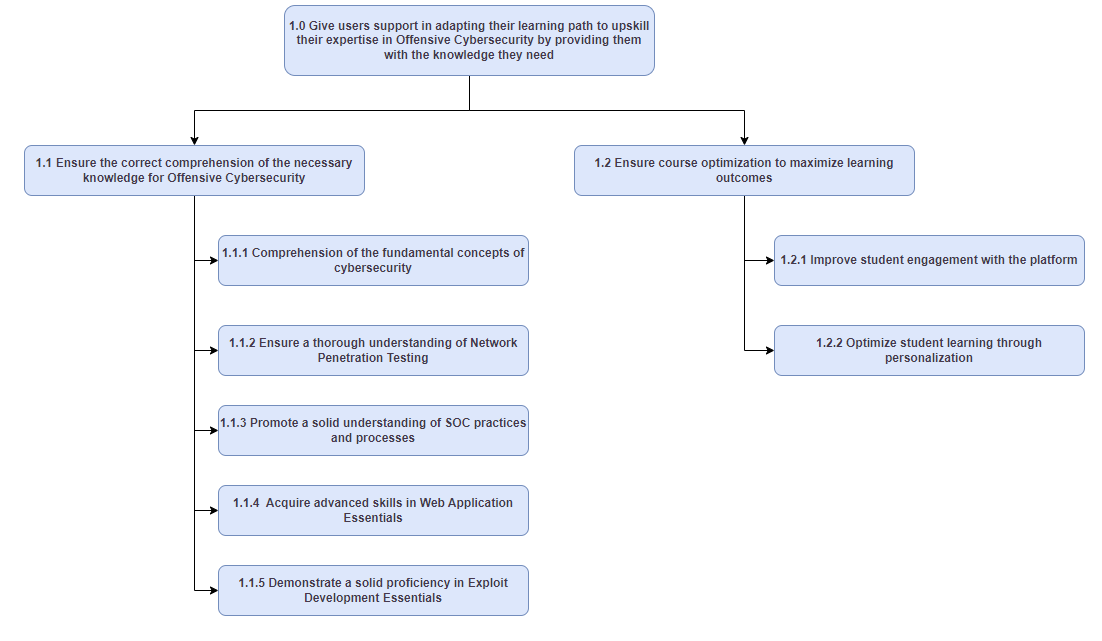
\includegraphics[width=\textwidth]{./assets/GDTA.png}
    \caption{Final GDTA Goal Tree}
    \label{fig:GDTA}
\end{figure}

The following sections will explain the details of each subgoal and their informational requirements, which are crucial for users to make informed decisions and achieve their objectives.
In order to fulfill a goal, a decision must be made based on the available information. We are not interested in trivial yes-or-no questions: instead, we are focusing on decisions that enable the fulfillment of high-level goals.

\newpage
\section{Major-Goal 1.1: Ensure the correct comprehension of the necessary knowledge for Offensive Cybersecurity}
In this section, we describe Major Goal 1.1 and its sub-goals.
The main aim of this goal, along with its sub-goals, is to outline the modules that users need to study to enhance their skills.

\subsection{Sub-Goal 1.1.1: Comprehension of the fundamental concepts of cybersecurity }
The objective of comprehending the fundamental concepts of cybersecurity is to provide individuals with a robust understanding of essential security principles and practices. Key areas of focus include ensuring confidentiality through mechanisms like OTP and MAC, maintaining data integrity with tools such as SHA256, and guaranteeing availability via digital signatures. Additionally, an understanding of blockchain technology and threat models is crucial, along with proficiency in cybersecurity algorithms and protocols like TLS. This foundational knowledge enables individuals to critically evaluate emerging technologies in relation to IT security and stay informed about current laws and regulations.

\begin{figure}[H]
    \centering
    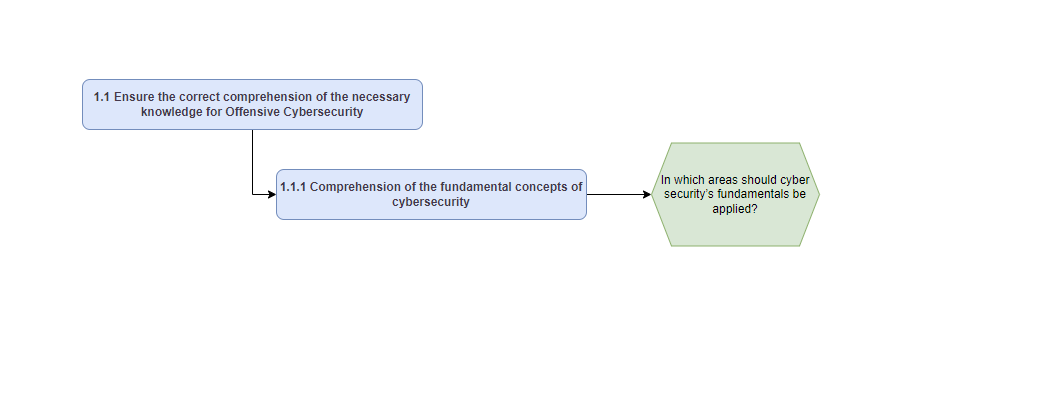
\includegraphics[width=\textwidth]{./assets/subgoal_1.1.1.png}
    \caption{Sub-Goal 1.1.1}
    \label{fig:subgoal_1.1.1}
\end{figure}

\begin{table}[H]
    \begin{center}
    \begin{tabular}{ | m{5cm} | m{5cm}| m{5cm} | } 
      \hline
      \textbf{Level 1 SA requirements} & \textbf{Level 2 SA requirements}  & \textbf{Level 3 SA requirements}  \\ 
      \hline
      CPA Security & Confidentiality & Capability to critically evaluate emerging technologies in relation to IT security, current laws and regulations\\ 
      \hline
      SHA256 & Integrity & \\ 
      \hline
      Advanced Schemes & Availability & \\ 
      \hline
      Zero Knowledge Proof &  Threat Models & \\ 
      \hline
      Blockchain & Algorithms for Cybersecurity  & \\ 
      \hline
      TLS Protocol &  & \\ 
      \hline
      Public Key&  & \\ 
      \hline
    \end{tabular}
    \end{center}
    \caption{SA requirements for subgoal 1.1.1}
    \end{table}
    
\newpage
\subsection{Sub-Goal 1.1.2: Ensure a thorough understanding of Network Penetration Testing}
The objective of ensuring a thorough understanding of network penetration testing is to equip individuals with the necessary skills and knowledge to effectively identify and mitigate security vulnerabilities within network infrastructures. This includes mastering fundamental programming concepts such as Python operators, syntax, and Powershell scripting, as well as understanding key network protocols like the Internet Protocol (IP) and Domain Name System (DNS). Advanced competencies involve applying cryptography techniques and hashing, acquiring in-depth Windows networking knowledge, and efficiently using variables, loops, and functions in Python and Powershell. Ultimately, this comprehensive understanding enables individuals to select the most appropriate penetration testing strategies for various scenarios, ensuring robust network security.

\begin{figure}[H]
    \centering
    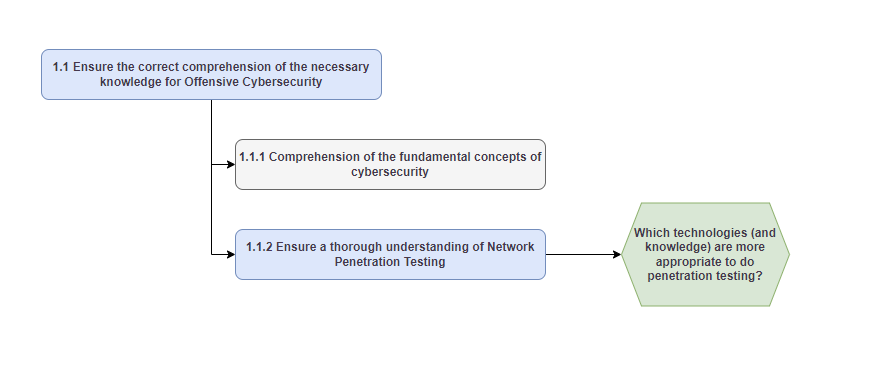
\includegraphics[width=\textwidth]{./assets/subgoal_1.1.2.png}
    \caption{Sub-Goal 1.1.2}
    \label{fig:subgoal_1.1.2}
\end{figure}

\begin{table}[H]
    \begin{center}
    \begin{tabular}{ | m{5cm} | m{5cm}| m{5cm} | } 
      \hline
      \textbf{Level 1 SA requirements} & \textbf{Level 2 SA requirements}  & \textbf{Level 3 SA requirements}  \\ 
      \hline
      Python operators & Cryptography techniques and hashing & Capability to choose the best penetration testing strategies based on the situation\\ 
      \hline
      Python syntax & Windows networking knowledge & \\ 
      \hline
      Powershell Scripting & Usage of variables & \\ 
      \hline
      Internet Protocol & Loops and functions in Python and Powershell  & \\ 
      \hline
      Domain Name System &  & \\ 
      \hline
    \end{tabular}
    \end{center}
    \caption{SA requirements for subgoal 1.1.2}
    \end{table}

\newpage
\subsection{Sub-Goal 1.1.3: Promote a solid understanding of SOC pratices and processes}
The objective of promoting a solid understanding of Security Operations Center (SOC) practices and processes is to provide individuals with the knowledge and skills necessary to effectively manage and respond to cybersecurity incidents. This includes foundational knowledge of network protocols such as the Internet Protocol (IP) and Domain Name System (DNS), as well as scripting skills with Powershell. Advanced competencies involve data conversion in Python between decimal, binary, and hexadecimal formats, understanding operational security and security management, and familiarity with practices such as the Cyber Kill Chain and logging. Ultimately, this comprehensive understanding enables individuals to proficiently detect and respond to cyber threats, ensuring robust security operations.

\begin{figure}[H]
    \centering
    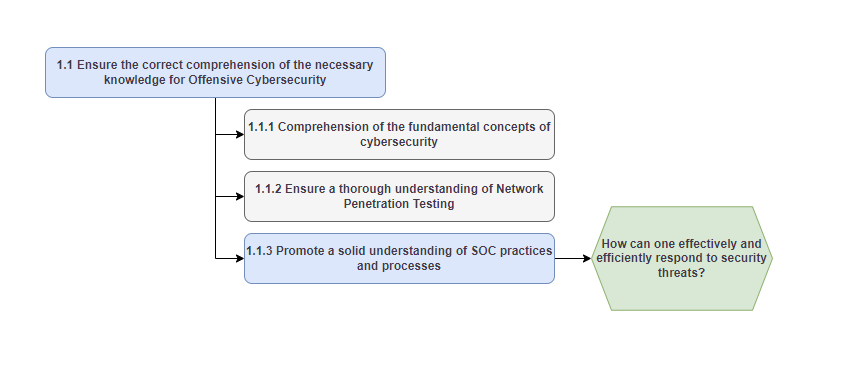
\includegraphics[width=\textwidth]{./assets/subgoal_1.1.3.png}
    \caption{Sub-Goal 1.1.3}
    \label{fig:subgoal1.1.3}
\end{figure}

\begin{table}[H]
\begin{center}
\begin{tabular}{ | m{5cm} | m{5cm}| m{5cm} | } 
  \hline
  \textbf{Level 1 SA requirements} & \textbf{Level 2 SA requirements}  & \textbf{Level 3 SA requirements}  \\ 
  \hline
  Internet Protocol & Data conversion in Python between decimal, binary, and hexadecimal & Knowing how to detect and respond to cyber threats\\ 
  \hline
  Powershell Scripting & Knowledge of operational security and security management & \\ 
  \hline
  Domain Name System & Practices of Cyber Kill Chain and Logging & \\ 
  \hline
  Firewall &  & \\ 
  \hline
\end{tabular}
\end{center}
\caption{SA requirements for subgoal 1.1.3}
\end{table}

\newpage
\subsection{Sub-Goal 1.1.4: Acquire advanced skills in Web Application Essentials}
The objective of acquiring advanced skills in web application essentials is to enable individuals to develop and maintain secure web applications. This encompasses foundational knowledge of web development technologies such as HTML, CSS, PHP, and JavaScript, along with proficiency in security tools like ZAP, AFL, SonarQube, and Flawfinder. Advanced skills include managing secure sessions, handling authentication, authorization, passwords, and cookies, and ensuring the security of REST, SOAP, and GraphQL services, as well as security practices in GIT. Ultimately, this comprehensive understanding equips individuals to recognize and mitigate vulnerabilities such as Server Side and Client Side XSS, Cross-Site Request Forgery, Clickjacking, and Content Sniffing, thereby ensuring robust web application security.

\begin{figure}[H]
    \centering
    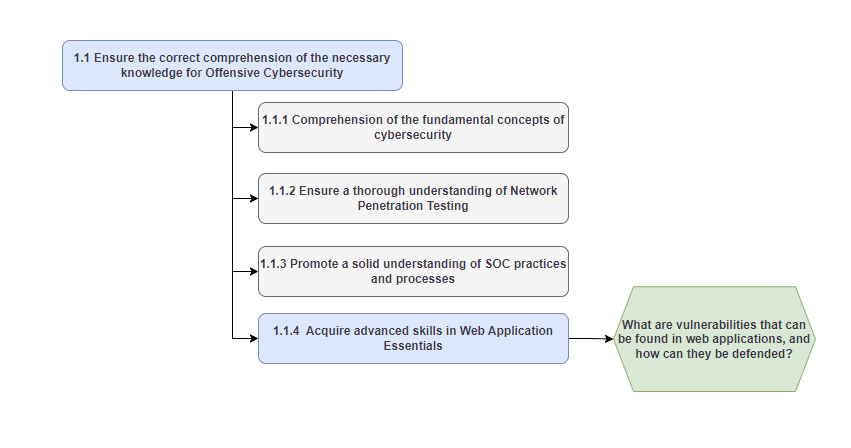
\includegraphics[width=\textwidth]{./assets/subgoal_1.1.4.png}
    \caption{Sub-Goal 1.1.4}
    \label{fig:subgoal1.1.4}
\end{figure}

\begin{table}[H]
\begin{center}
\begin{tabular}{ | m{5cm} | m{5cm}| m{5cm} | } 
  \hline
  \textbf{Level 1 SA requirements} & \textbf{Level 2 SA requirements}  & \textbf{Level 3 SA requirements}  \\ 
  \hline
  HTML, CSS, PHP, Javascript & Managing secure sessions, including authentication, authorization, passwords, and cookies, REST, SOAP and GraphQL services, security in GIT & Understanding how to make a secure web application\\ 
  \hline
  ZAP &  & Recognizing Server Side \& Client Side XSS, Cross-Site Request Forgery, Clickjacking, Content Sniffing\\ 
  \hline
  AFL &  & \\ 
  \hline
  SonarQube, Flawfinder &  & \\ 
  \hline
\end{tabular}
\end{center}
\caption{SA requirements for subgoal 1.1.4}
\end{table}

\newpage
\subsection{Sub-Goal 1.1.5: Demonstrate a solid proficiency in Exploit Development Essentials}
The objective of demonstrating solid proficiency in exploit development essentials is to enable individuals to effectively identify and develop exploits for various security vulnerabilities. This includes foundational knowledge of network protocols, VPNs, and firewalls. Advanced competencies involve understanding ARM-32 and ARM-64 assembly, manipulating registers, stacks, and functions, and analyzing binary files. Ultimately, this comprehensive skill set allows individuals to understand how malicious scripts affect applications, identify flaws in security measures, and leverage exploit frameworks to enhance cybersecurity defenses.

\begin{figure}[H]
  \centering
  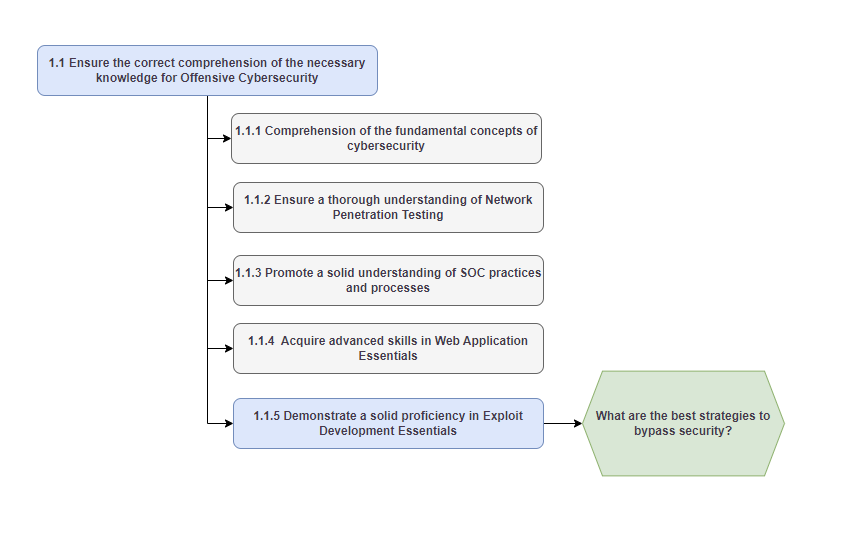
\includegraphics[width=\textwidth]{./assets/subgoal_1.1.5.png}
  \caption{Sub-Goal 1.1.5}
  \label{fig:subgoal1.1.5}
\end{figure}

\begin{table}[H]
    \begin{center}
    \begin{tabular}{ | m{5cm} | m{5cm}| m{5cm} | } 
      \hline
      \textbf{Level 1 SA requirements} & \textbf{Level 2 SA requirements}  & \textbf{Level 3 SA requirements}  \\ 
      \hline
      Network Protocols & Assembly for ARM-32 and ARM-64 & Understanding how a malicious script affects an application\\ 
      \hline
      VPN &  Registers, stacks and functions & Ability to identify flaws in security measures\\ 
      \hline
      Firewalls & Analysis of binary files & Knowledge of exploits frameworks\\  
      \hline
    \end{tabular}
    \end{center}
    \caption{SA requirements for subgoal 1.1.5}
    \end{table}

\newpage
\section{Major Goal 2.1: Ensure course optimization to maximize learning outcomes}
This Major-Goal aims to make the platform more engaging and effective for users. It focuses on two main things: boosting how users interact with the platform and making studying more personalized based on how each user learns.

To achieve this, the platform will track how users use it—what they are interested in, what skills they have, and where they might need help. With this info, the platform can adjust how it works to match each user's progress and preferences. 

\subsection{Sub-Goal 1.2.1: Improve student engagement with the platform}
The objective of improving student engagement with the platform focuses on increasing and enhancing student interactions. Key metrics include session length, number of active users, days spent on module, forum activity (questions and answers) and the engagement level with the platform. The analysis of these data involve user's session length compared with the length of other users session, a comparison between the days spent on a module by students, and student interaction within the forum. Ultimately, the goal is to prevent student dropout by understanding and addressing engagement factors.

\begin{figure}[H]
    \centering
    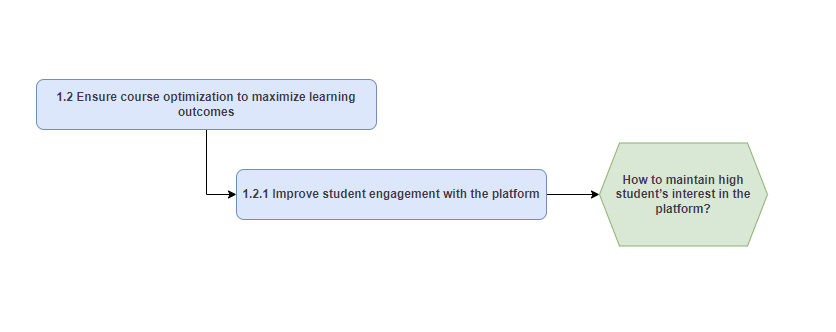
\includegraphics[width=\textwidth]{./assets/subgoal_1.2.1.png}
    \caption{Sub-Goal 1.2.1}
    \label{fig:subgoal1.2.1}
\end{figure}

\begin{table}[H]
\begin{center}
\begin{tabular}{ | m{5cm} | m{5cm}| m{5cm} | } 
  \hline
  \textbf{Level 1 SA requirements} & \textbf{Level 2 SA requirements}  & \textbf{Level 3 SA requirements}  \\ 
  \hline
  Number of active users &  Comparison between students session lengths & Preventing student dropout \\ 
  \hline
  Session length & Comparison between days spent on module by students & \\ 
  \hline
  Days spent on module & Student interaction within the forum & \\
  \hline
  Number of answers on the forum &  & \\ 
  \hline
  Number of questions on the forum &  & \\ 
  \hline
  Number of notifications on the forum &  & \\ 
  \hline
  Engagement Level & & \\ 
  \hline
\end{tabular}
\end{center}
\caption{SA requirements for subgoal 1.2.1}
\end{table}

\newpage
\subsection{Sub-Goal 1.2.2: Optimize student learning through personalization}
The objective of optimizing student learning through personalization is to enhance educational effectiveness by tailoring the learning experience to individual student needs and preferences. This involves assessing student performance through end-of-module assessments and tracking course completion. Additionally, it requires analyzing trends in student performance over time to identify areas for improvement. Furthermore, the initiative aims to optimize learning by monitoring the used resources, identifying areas of difficulty and preferred learning styles, and evaluating the acquisition of specific skills. By leveraging these insights, the goal is to create a more personalized educational environment that supports and enhances student learning outcomes effectively.
\begin{figure}[H]
    \centering
    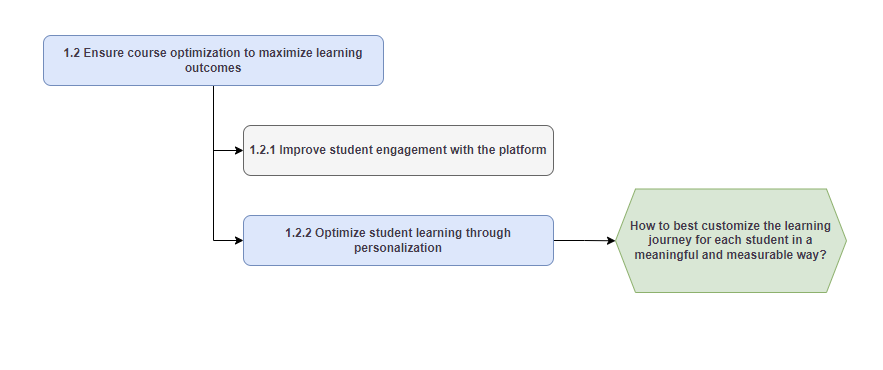
\includegraphics[width=\textwidth]{./assets/subgoal_1.2.2.png}
    \caption{Sub-Goal 1.2.2}
    \label{fig:subgoal1.2.2}
\end{figure}

\begin{table}[H]
\begin{center}
\begin{tabular}{ | m{5cm} | m{5cm}| m{5cm} | } 
  \hline
  \textbf{Level 1 SA requirements} & \textbf{Level 2 SA requirements}  & \textbf{Level 3 SA requirements}  \\ 
  \hline
  End-of-module test scores & Percentage of completed course & Trends in student performance over time \\ 
  \hline
  Modules visited & Problem-Solving vs Memory Performance & \\ 
  \hline
  Used material & Percentage of usage of the different kinds of materials provided to the students showing their preferences & \\ 
  \hline
   & Skill types and areas of difficulty & \\ 
  \hline
\end{tabular}
\end{center}
\caption{SA requirements for subgoal 1.2.2}
\end{table}